\subsection{Arsitektur yang Mengoptimalkan PostgreSQL (PGP)}

Arsitektur ini mengoptimalkan sistem dengan pola CQRS, pola penyeimbangan beban berbasiskan antrean, dan menggunakan ekstensi Citus untuk menjalankan basis data secara terdistribusi.

\begin{figure}[htbp]
    \centering
    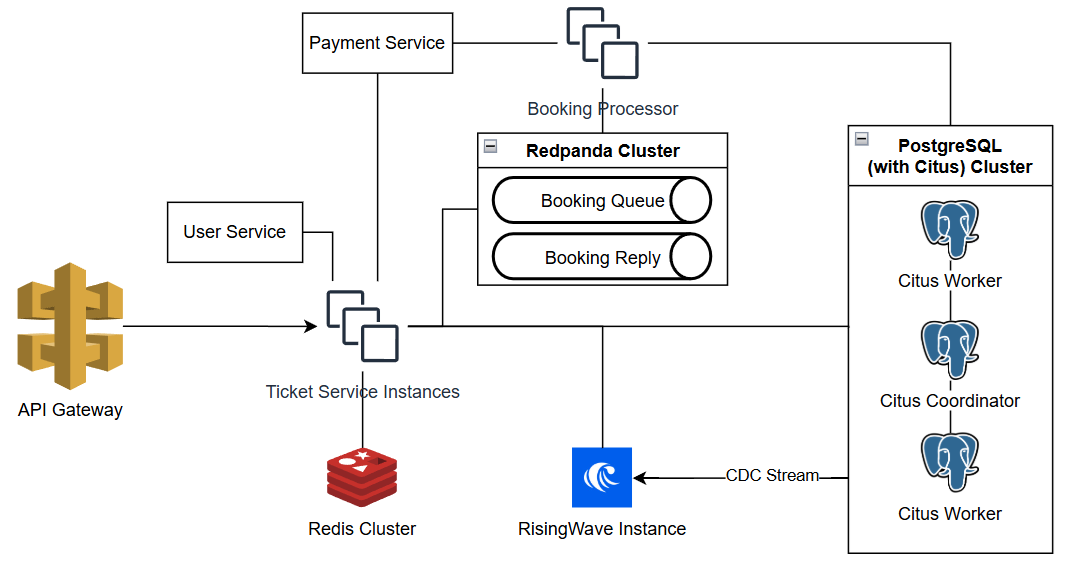
\includegraphics[width=1\textwidth]{resources/appendix/architecture-optimized.png}
    \caption{Arsitektur yang Mengoptimalkan PostgreSQL}
    \label{fig:optimized-architecture}
\end{figure}

\subsubsection{Peningkatan \textit{Throughput} PostgreSQL dengan Citus}

Penggunaan ekstensi Citus memungkinkan peningkatan \textit{throughput} dengan pendekatan \textit{scale-out}. Peningkatan ini tidak hanya pada \textit{throughput} baca, tetapi juga \textit{throughput} tulis. Hal ini dapat dicapai dengan pembagian data pada tabel berdasarkan baris, lalu setiap \textit{node} yang memegang bagian data tersebut dibuat menjadi \textit{writer}.

\textit{Sharding} berdasarkan baris dapat dilakukan pada tabel Seats, IssuedTicket, OrderItem, dan Orders. Entitas sisanya dapat dibuat sebagai tabel yang direplikasi ke setiap node.

\subsubsection{Penggunaan Pola Penyeimbangan Beban dengan Antrean}

Perintah pemesanan tiket (berupa \textit{command}/ \textit{event sourcing}) akan dimasukkan ke dalam antrean Redpanda terlebih dahulu. Lalu, \textit{booking processor} akan memproses permintaan secara bertahap berdasarkan kemampuan sistem. Pendekatan ini memungkinkan terjaganya stabilitas sistem ketika terdapat \textit{burst request}.

Selain itu, akan lebih baik apabila sistem dapat menolak permintaan pesanan lebih awal, seperti karena sudah ada pesanan yang sedang diproses tetapi masih belum \textit{commit}. Hal ini dapat didukung dengan penggunaan Redis untuk menyimpan \textit{uncommited data} yang akan digunakan untuk menolak permintaan pesanan lebih awal.

\begin{figure}[htbp]
    \centering
    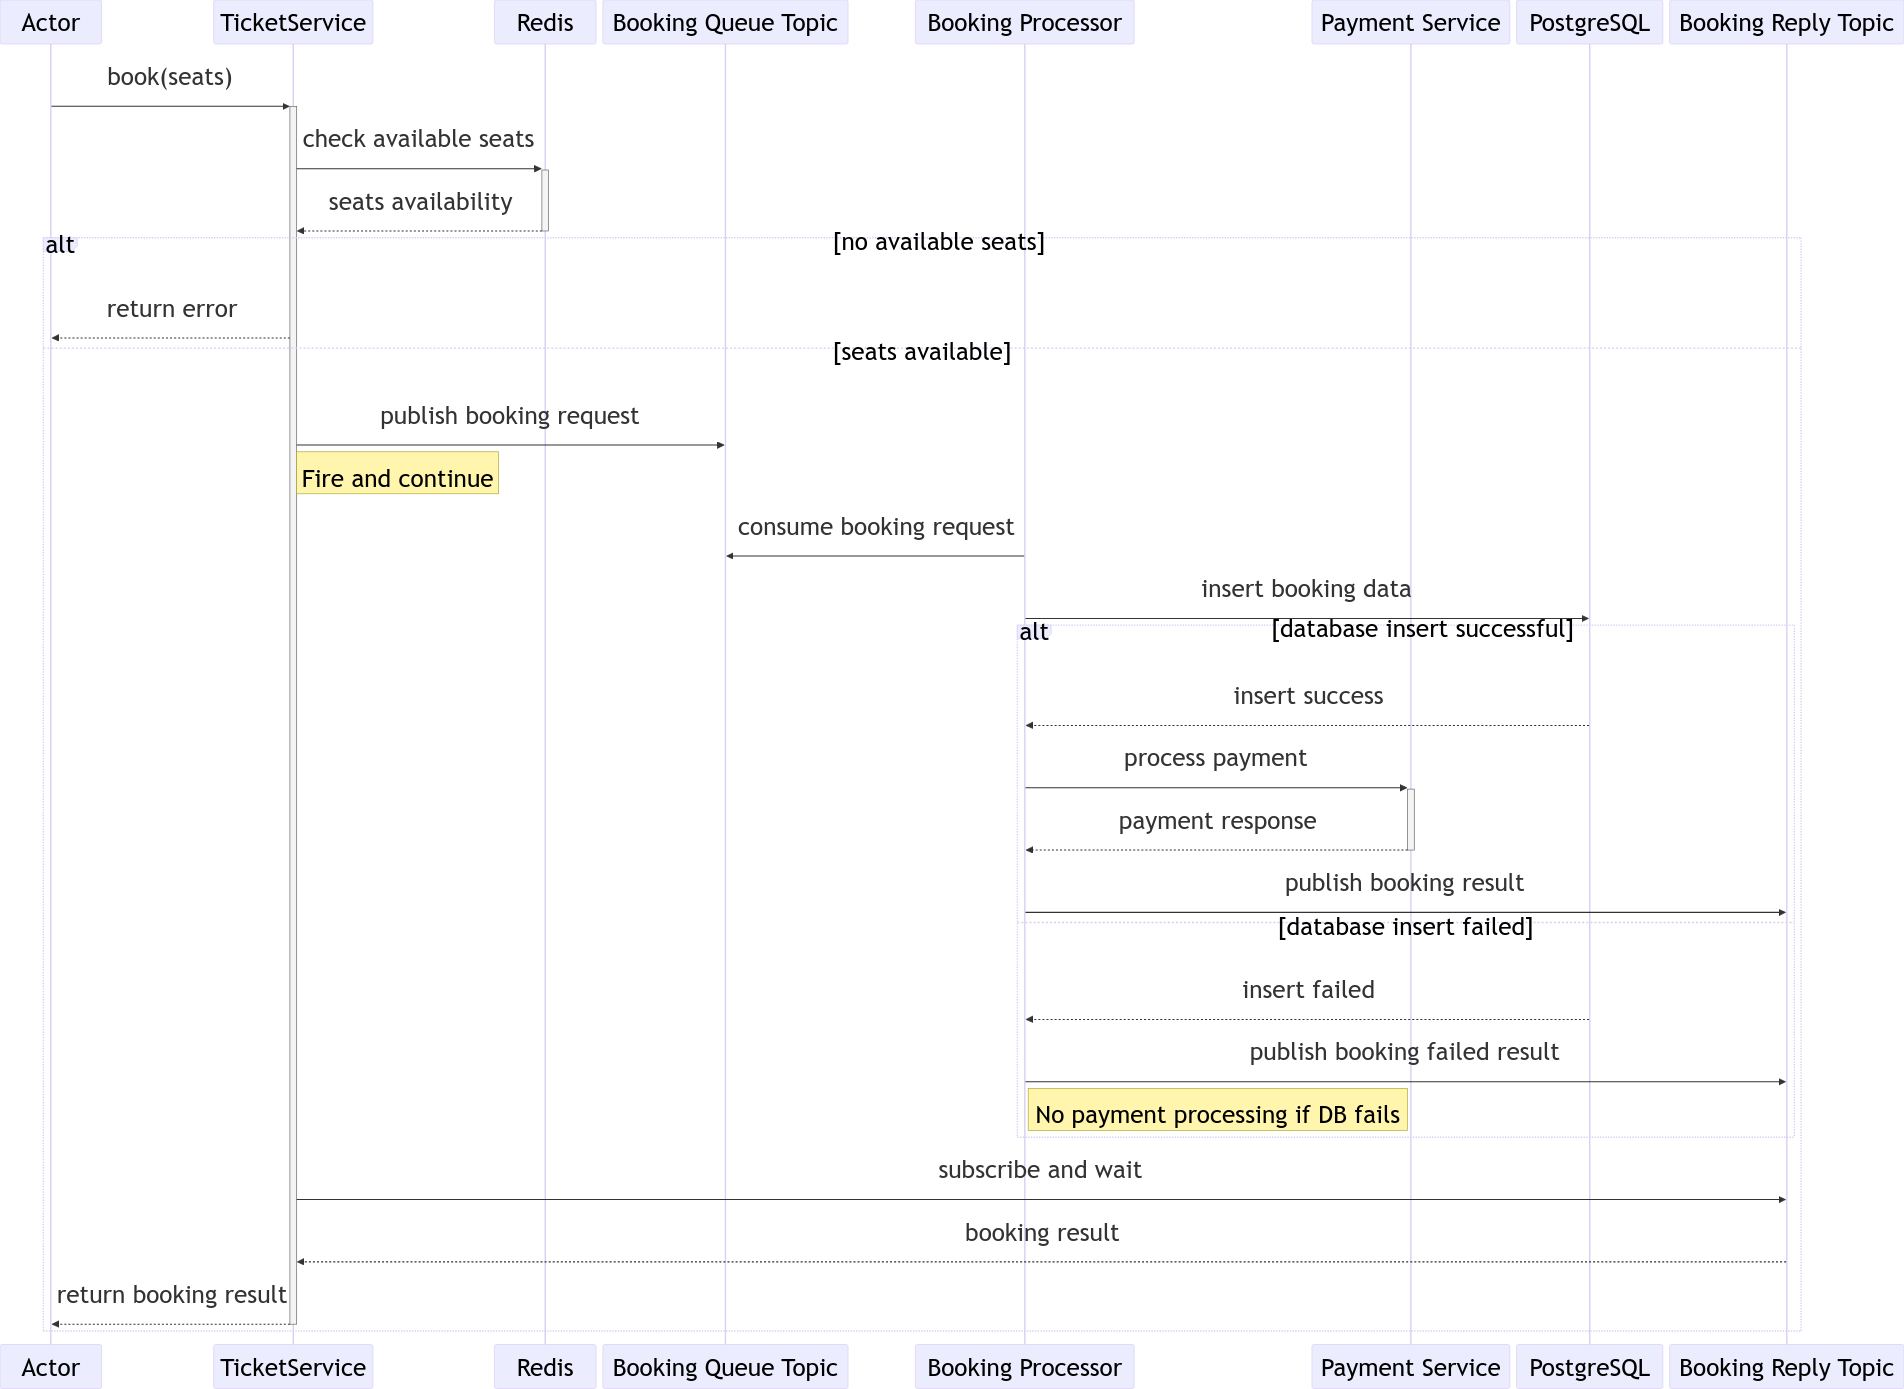
\includegraphics[width=1\textwidth]{resources/appendix/pgp-purchase-flow.png}
    \caption{Alur Pemesanan Tiket Pada PGP}
    \label{fig:pgp-purchase-flow}
\end{figure}

Terdapat dua isu yang harus dibahas pada pendekatan ini, yaitu:

\begin{enumerate}
    \item \textit{Persistence} pada Redis bersifat asinkron, sehingga terdapat kemungkinan data hilang ketika terjadi kegagalan. Meskipun begitu, penggunaan \textit{key-value store} lain yang \textit{persistent} berpotensi memperlambat kinerja. Dalam kasus ini, Redis akan dikonfigurasikan dalam mode kluster untuk penskalaan secara horizontal dan kombinasi antara \textit{snapshot} dan AOF untuk \textit{persistence}. Hilangnya data dapat terjadi ketika terdapat \textit{node} yang mengalami kegagalan. Meskipun begitu, \textit{data loss} atau \textit{eventual consistency} tidak akan mengganggu integritas sistem karena masih akan ada validasi lagi ketika pemrosesan pesanan.
    \item Isu \textit{fairness} harus diperhatikan ketika menggunakan Redpanda sebagai antrean. Redpanda hanya menjamin \textit{ordering} dalam satu partisi yang sama dan tidak menjamin \textit{ordering} secara global dalam satu topik. Salah satu cara untuk memastikan \textit{fairness} adalah dengan melakukan pembagian/ pemartisian antrean berdasarkan kategori tiket. Dengan begitu, pemrosesan pada antrean akan sesuai dengan urutan permintaan. Meskipun begitu, pendekatan ini mengharuskan pembelian lebih dari satu tiket dalam satu waktu hanya mendukung pemesanan dalam satu kategori yang sama.
    \item Dengan menggunakan antrean, komunikasi akan menjadi asinkron. Untuk menghubungkan permintaan dan respons, \textit{correlation id} dapat digunakan. Terdapat dua alternatif agar pengguna dapat diberitahu agar mendapatkan respons, yaitu menggunakan \textit{notify} dari sisi server atau respons pemesanan baru akan diberikan ketika sudah terdapat respons. Pendekatan yang dipilih adalah pendekatan kedua karena permintaan pemesanan juga membutuhkan aksi lanjutan untuk proses pembayaran. Selain itu, \textit{latency} pemrosesan permintaan ini juga dapat berguna sebagai \textit{metrics} dalam pengujian.
\end{enumerate}

\subsubsection{Pelimpahan Tanggung Jawab Baca Kepada RisingWave}

Pada permintaan baca ketersediaan tiket, tanggung jawab penanganannya dapat dilimpahkan kepada RisingWave. \textit{Streaming database} ini mengonsumsi \textit{CDC stream} dari kluster PostgreSQL, lalu memperbarui kueri secara inkremental. Dengan begitu, operasi baca tidak akan membebani basis data dan penanganannya dapat dilakukan dengan lebih efisien dengan RisingWave.

Sama seperti penggunaan \textit{read replica}, hal yang harus diperhatikan dalam penggunaan RisingWave adalah \textit{replication lag}. Data yang dikembalikan oleh RisingWave tidak valid apabila data tersebut \textit{outdated}. Pendekatan ini tidak mendukung konfigurasi agar transaksi \textit{commit} setelah RisingWave \textit{acknowledge} data, sehingga tetap akan ada \textit{replication lag}. Solusi dari permasalahan ini adalah \textit{tuning} RisingWave agar mampu mengikuti beban yang dikirimkan oleh PostgreSQL.

\subsubsection{Penskalaan Pada PGP}

Berikut adalah strategi penskalaan untuk setiap komponen selain dengan pendekatan \textit{scale-up}:

\begin{enumerate}
    \item Layanan tiket dapat di-\textit{scale} dengan menambah jumlah \textit{instance}.
    \item Redis dapat di-\textit{scale} dengan menggunakan konfigurasi kluster, sehingga data di-\textit{shard} berdasarkan \textit{range} hash. Penskalaan ini memungkinkan peningkatan \textit{throughput} untuk operasi baca dan tulis.
    \item Pemroses pesanan dapat di-\textit{scale} dengan menambah jumlah \textit{instance}. Jumlah pemroses ini mengikuti jumlah partisi pada topik.
    \item RisingWave dapat di-\textit{scale} dengan meningkatkan jumlah \textit{instance}. RisingWave dapat secara otomatis mengatur penggunaan sumber daya sehingga mampu menggunakan seluruh sumber daya yang tersedia.
    \item Kluster Redpanda dapat di-\textit{scale} dengan menggunakan beberapa partisi. Setiap partisi akan menangani permintaan untuk satu atau beberapa kategori tiket yang telah ditentukan. Jumlah partisi permintaan dan respons akan sama.
\end{enumerate}

\subsubsection{Aspek Lain}

\begin{enumerate}
    \item Pendekatan pemartisian berdasarkan kategori mengharuskan konfigurasi dilakukan secara manual setiap kali akan diadakan proses penjualan. Mekanisme atau analisis yang memungkinkan konfigurasi secara otomatis tidak akan dibahas karena di luar \textit{scope} penelitian ini.
    \item Penggunaan PostgreSQL dan kakas lain yang \textit{out of the box} memiliki banyak fitur memungkinkan \textit{extendability} yang lebih baik dengan kompleksitas yang tidak sebesar solusi EDA.
    \item Pada saat penjualan, dapat diasumsikan entitas Events, TicketCategory, Areas, TicketSale, dan TicketPackage tidak berubah sehingga data entitas tersebut dapat di-\textit{cache}.
\end{enumerate}